%!TEX root = ../dissertation.tex

\chapter[ChapterShortTitle]{ChapterTitle}

Now let's walk through some \textbackslash ref commands:

\begin{exe}
    \ex \textbackslash ref: \ref{chap:Intro}
    \ex \textbackslash autoref: \autoref{chap:Intro}
    \ex \textbackslash eqref: \eqref{chap:Intro}
    \ex \textbackslash nameref: \nameref{chap:Intro}
    
\end{exe}

\todo{an example of the default todo note}

Adding an image:
\begin{figure}[ht]
    \centering
    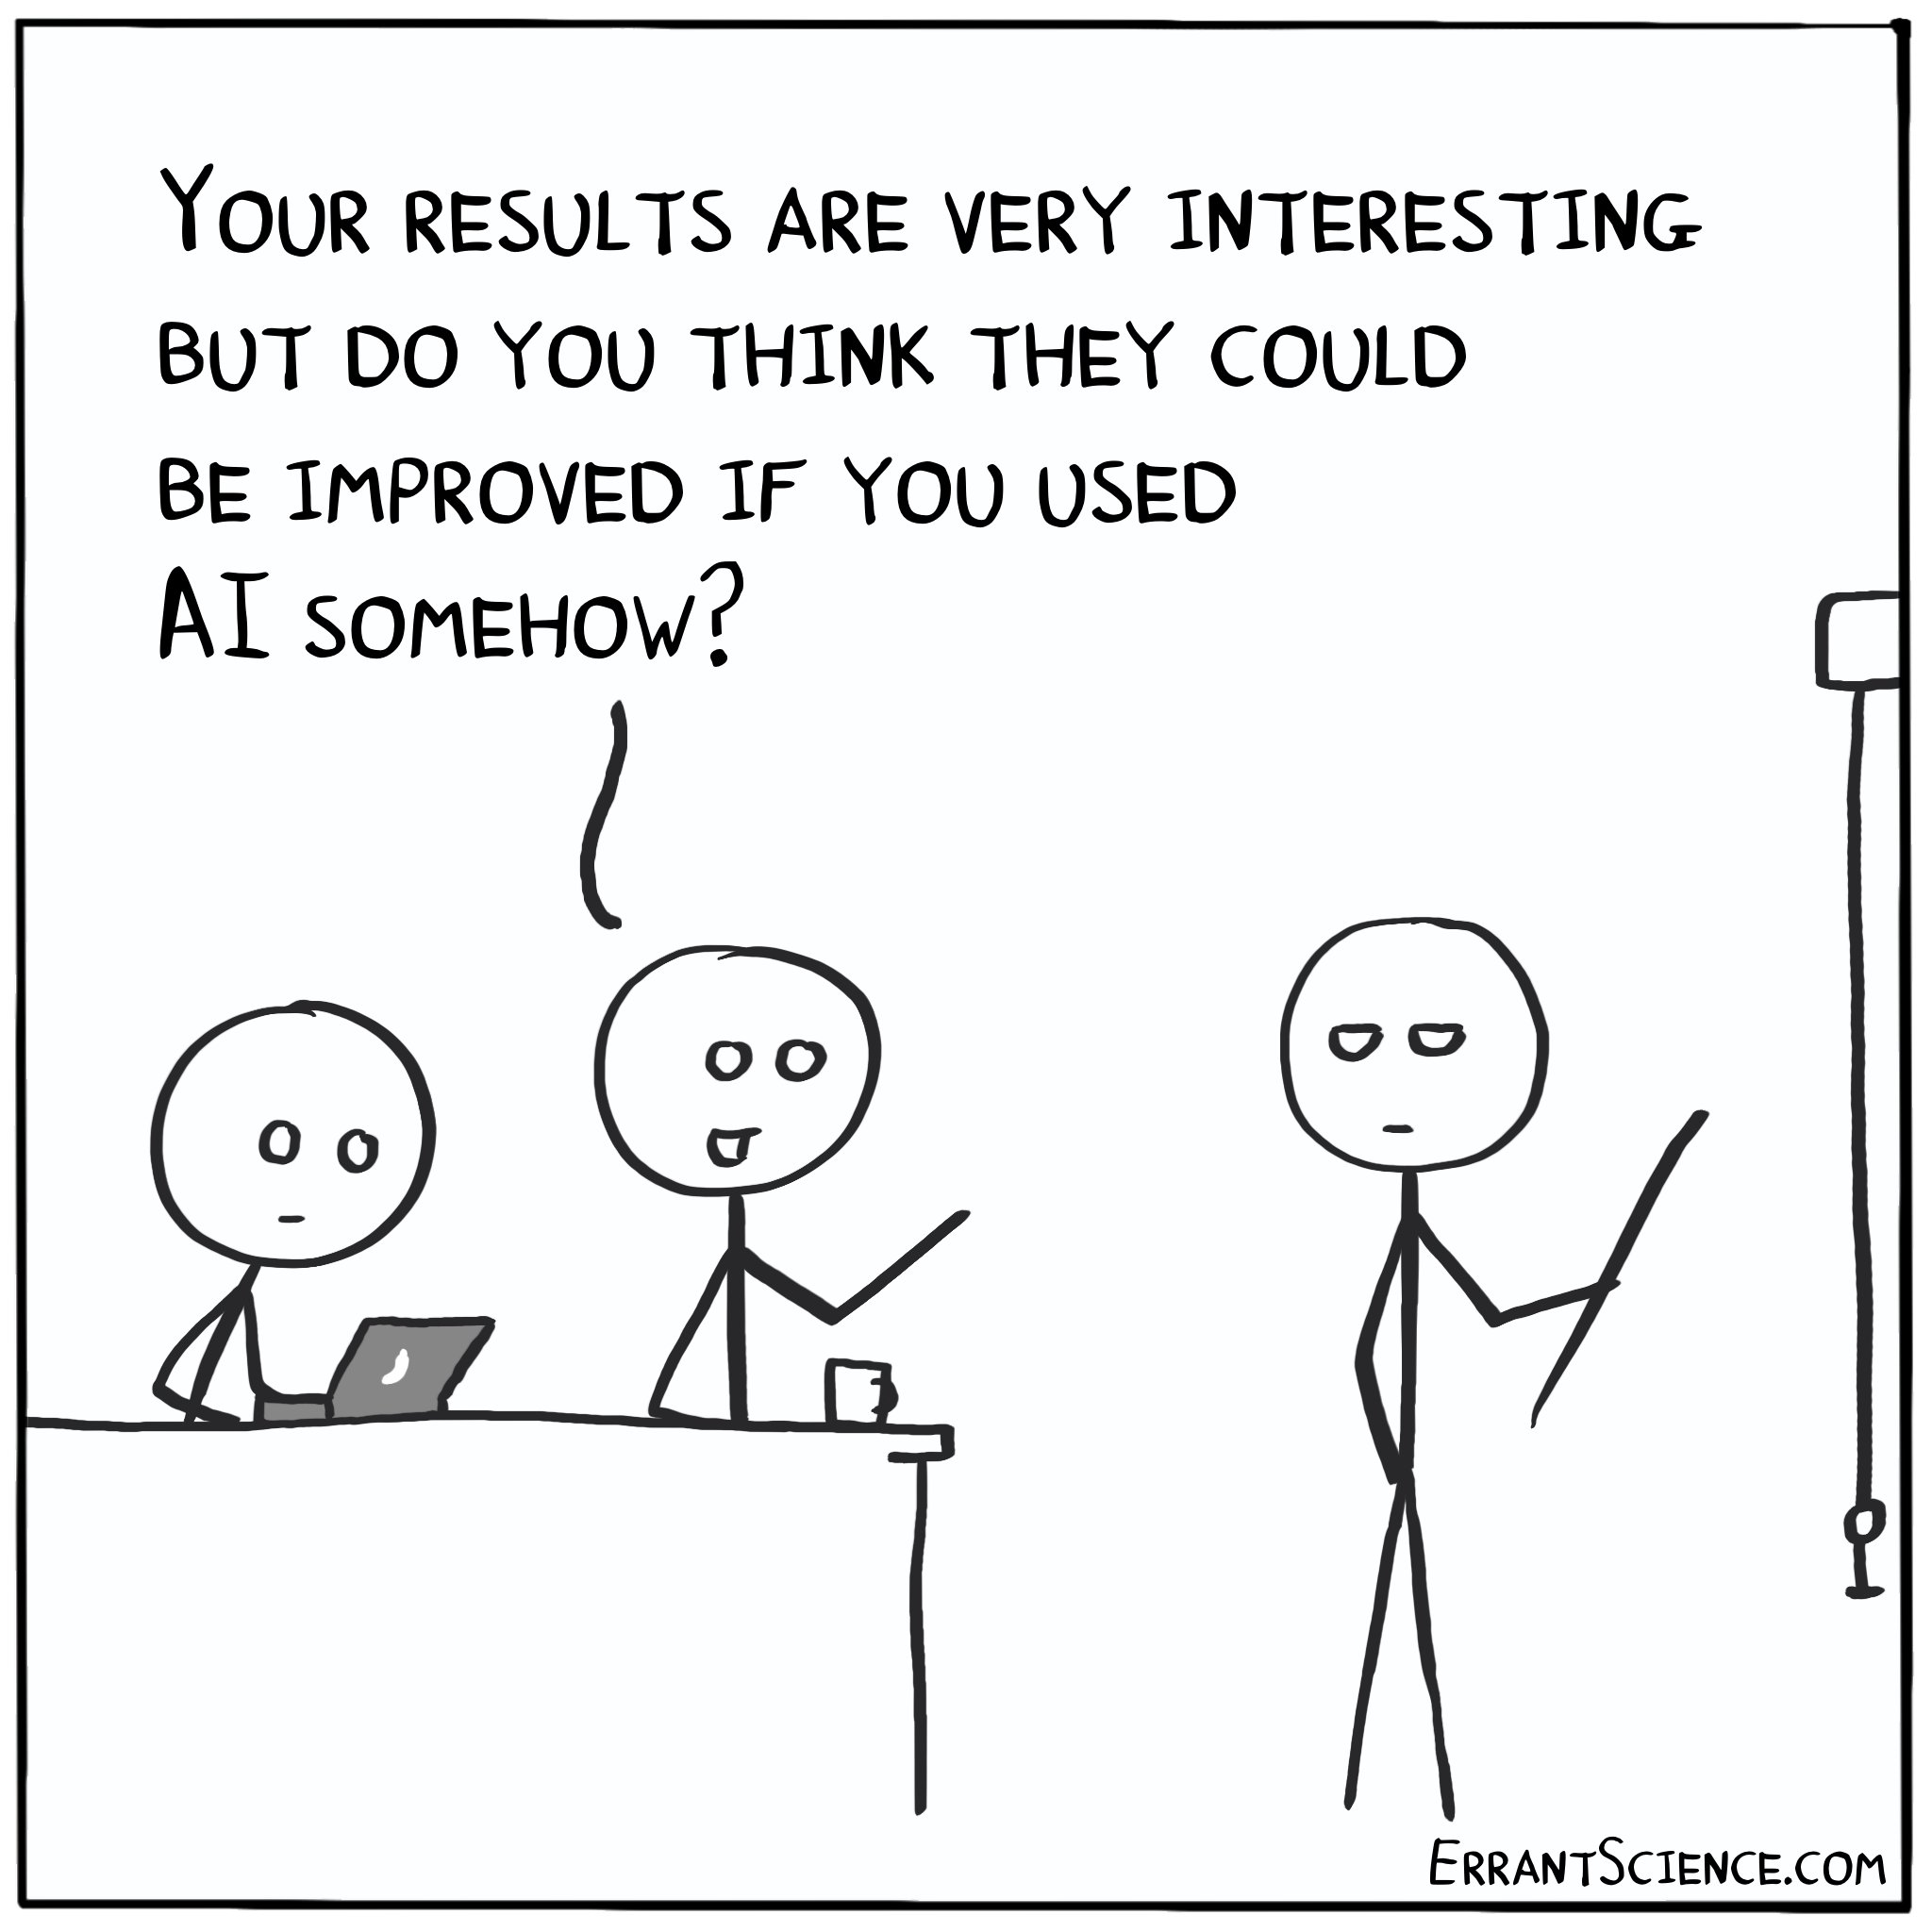
\includegraphics[width=0.45\textwidth]{images/ai-results-improve.jpeg}
    \caption{Sample Image}
    \label{fig:ai-image}
\end{figure}

Adding a panel of images:
\begin{figure}[ht]
    \begin{minipage}[b]{0.48\textwidth}
        \centering
        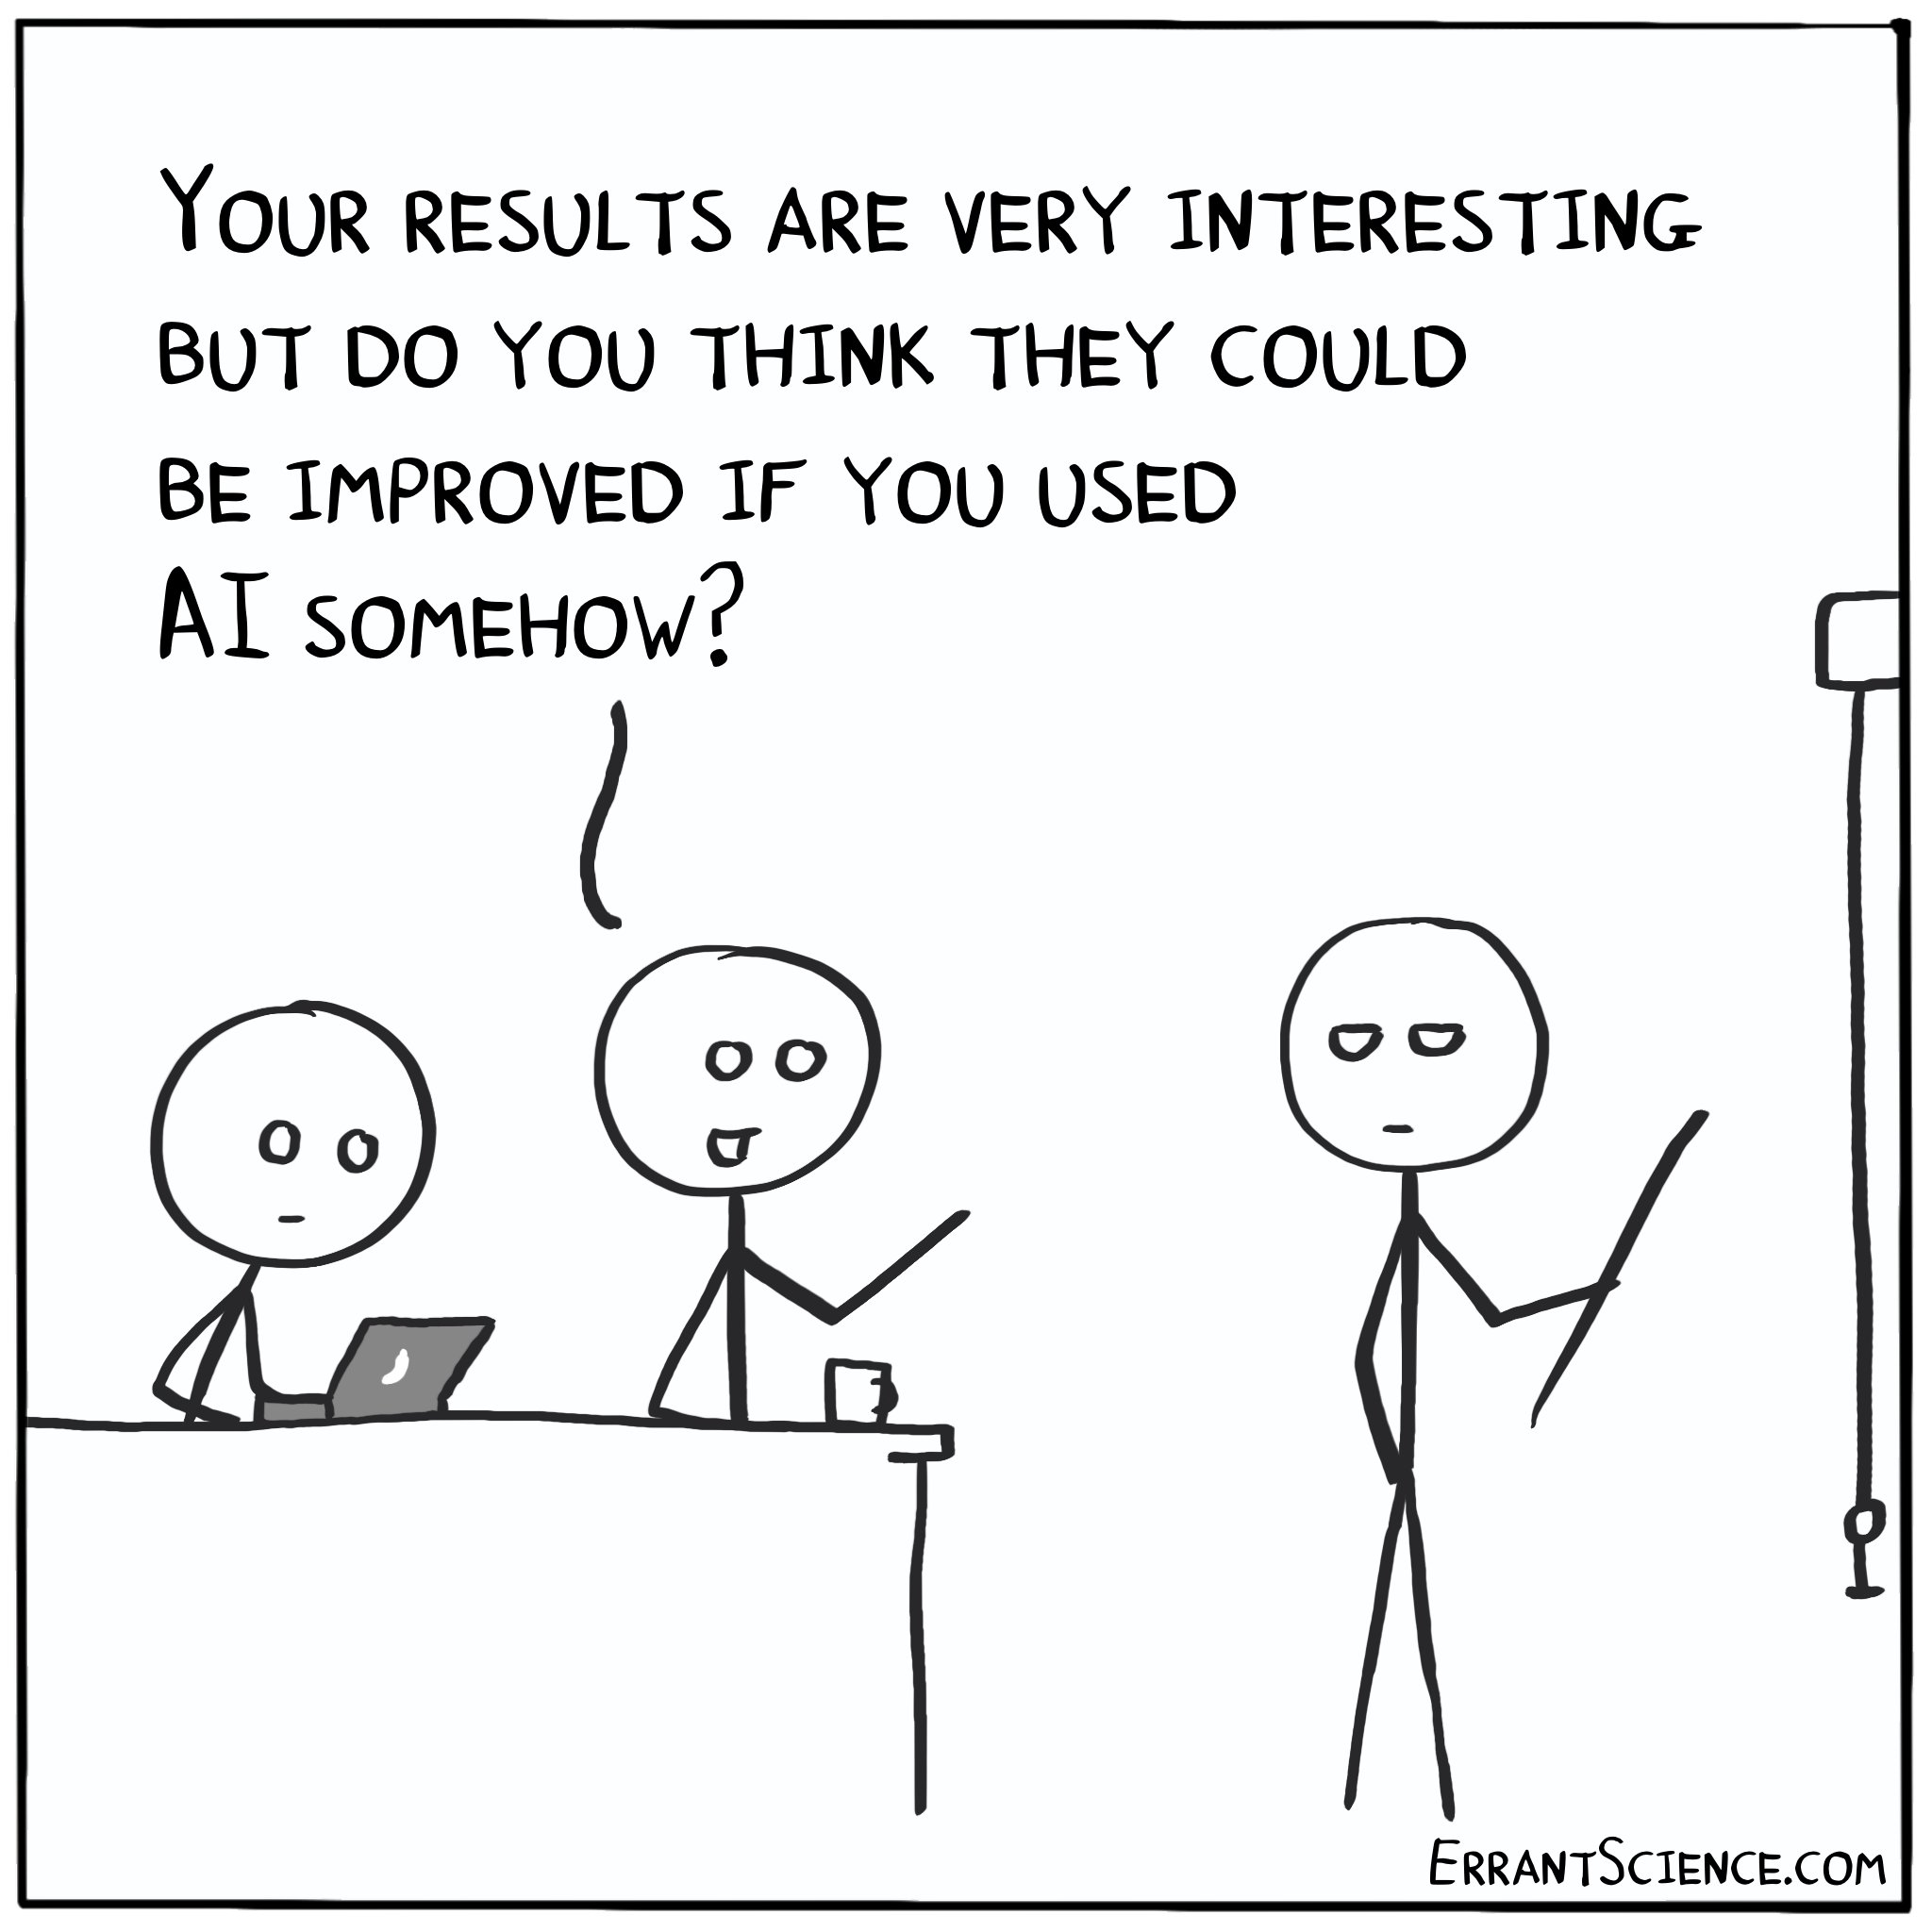
\includegraphics[width=\textwidth]{images/ai-results-improve.jpeg}
        \caption{Image One}
        \label{fig:image-one}
    \end{minipage}
    % \hspace{0.1cm}
    \begin{minipage}[b]{0.48\textwidth}
        \centering
        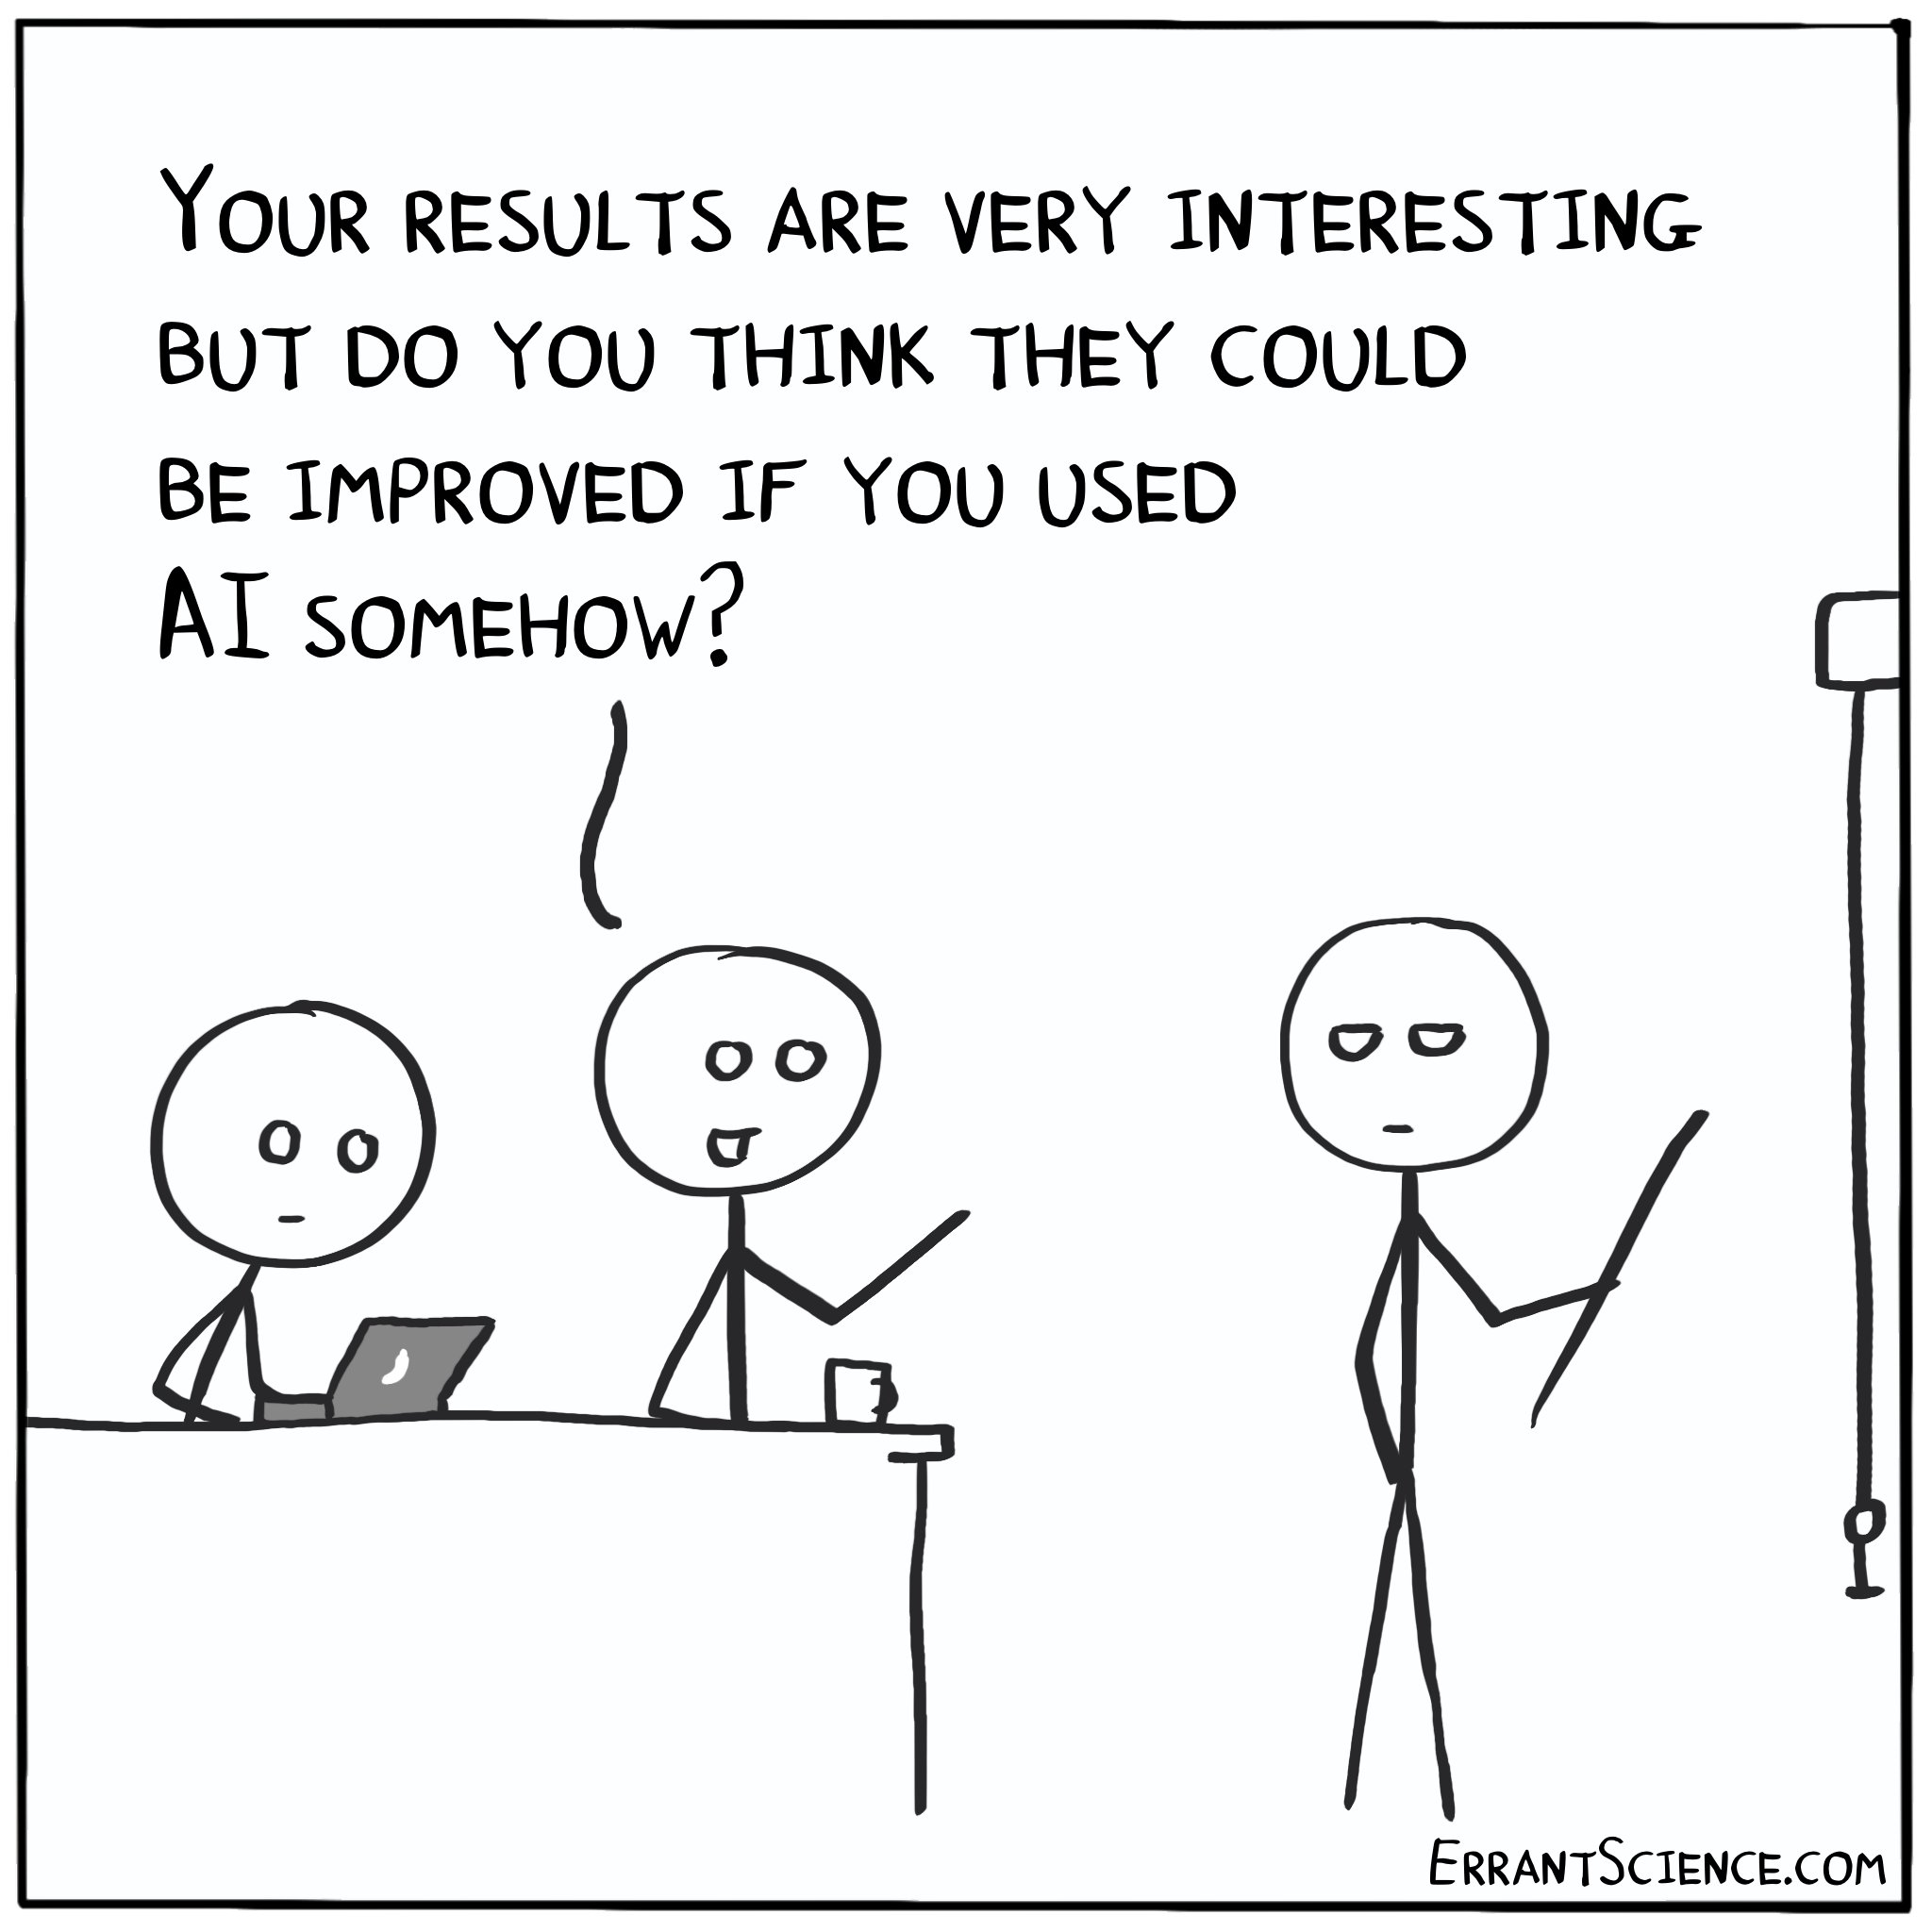
\includegraphics[width=\textwidth]{images/ai-results-improve.jpeg}
        \caption{Image 2}
        \label{fig:image-two}
    \end{minipage}
\end{figure}
